\documentclass[conference]{IEEEtran}
\IEEEoverridecommandlockouts
\usepackage{cite}
\usepackage{amsmath,amssymb,amsfonts}
\usepackage{newtxtext,newtxmath}
\usepackage{graphicx}
\usepackage{textcomp}
\usepackage{xcolor}
\usepackage{booktabs}
\usepackage{url}
\usepackage{hyperref}
\usepackage{multirow}
\usepackage{balance}

\graphicspath{{figures/}{paper/figures/}}

\hypersetup{
    colorlinks=true,
    linkcolor=black,
    citecolor=black,
    urlcolor=blue
}

\begin{document}

\title{A Dual-Layer Framework for LLM Prompt Injection Detection and Security}

\author{\IEEEauthorblockN{Omika Shrestha, Diksha Jha, Neda Nizamudeen, Jesline Pinto}
\IEEEauthorblockA{\textit{Department of Computer Science \& Engineering} \\
\textit{Symbiosis Institute of Technology, Symbiosis International (Deemed University)} \\
Pune, India \\
Project Guide: Mrs. Usha Anirudhha Jogalekar, Assistant Professor \\
Implementation repository: \url{https://github.com/jhadiksha65/prompt-injection-detector}}
}

\maketitle

\begin{abstract}
Prompt injection poses a threat to applications that mix trusted code with untrusted user input, uploaded files and external content. This paper introduces a two-layer security architecture that incorporates inbound neural--heuristic screening and outbound response sanitization. The inbound layer combines a highly optimized DistilBERT classifier, deterministic rules, a nine-category threat taxonomy and attachment-specific processing for supported attachments, such as OCR for raster images. The outbound layer scans completed model answers for possible prompt disclosure, credential-like strings, personally identifiable information (PII), and structural anomalies before sending them out. An OpenAI-compatible gateway that blocks pre-execution, no LLM invocations on tested blocked paths, buffers responses for inspection prior to server-sent-event delivery. The hybrid detector yields 99.03\% accuracy, 99.26\% precision, 98.80\% recall and an F1-score of 0.9903 on the 3,000-example generalization test. It has a 99.17\% accuracy and 98.33\% recall on a 600 example challenge holdout set, and no false positives out of the 300 benign examples in the holdout set. There are 288 tests in 20 modules in the implementation's regression suite. These results show the success of the approach of using neural classification, deterministic rules, attachment processing, and output inspection on the datasets evaluated.
\end{abstract}

\begin{IEEEkeywords}
prompt injection, large language model security, DistilBERT, rule-based detection, output filtering, attachment parsing, defense in depth
\end{IEEEkeywords}

\section{Introduction}
Large language model (LLM) applications are increasingly ingesting user instructions along with retrieved web pages, uploaded documents, outputs from tools, and other untrusted content. Prompt injection takes advantage of this by embedding instructions within the content that the model might consider authoritative. Direct attacks are made through the user facing prompt, and indirect attacks are made through external content like documents or web pages [1]--[4]. Successful attack can result in a redirection of a model's task, affect tool use, or try to gain confidential context.

A single input filter is not enough to solve prompt injection. Keyword rules are simple to interpret, easy to implement, but can be ineffective at detecting paraphrases and can trigger false alarms for non-attack-related conversations. Neural classifiers can identify more general language patterns, but are sensitive to composition and distribution shift in the data sets. Furthermore, the input filtering does not allow to check the output of the model itself. Previous research on prompt-injection attacks and agent benchmarks encourages considering not only detection quality but also application-level enforcement [2]--[8] when evaluating an attack. Prompt injection and disclosure of sensitive information are also highlighted as risks in the OW ASP GenAI guidance [12].

This paper describes the middleware architecture implemented and the evaluation of the detection performance, attachment-processing behavior, application-level enforcement, and response-inspection pipeline of the implemented middleware architecture based on the project benchmark sets and automated integration tests.

\subsection{Contributions}
The paper makes four contributions:
\begin{itemize}
    \item It describes an inbound screening pipeline that combines a DistilBERT-based classifier with deterministic rule signals and a threat taxonomy.
    \item It documents separate processing paths for user prompts and supported attachments, including OCR for raster images, to help identify the source of suspicious content.
    \item It describes outbound response checks for suspected prompt disclosure, credential-like strings, PII, and structural anomalies.
    \item It reports confusion-matrix-derived results for three evaluation sets, summarizes the automated regression suite, and reports the measured detection, integration-test, and middleware-latency results.
\end{itemize}

\subsection{Research Questions}
We examine four questions: (RQ1) how does hybrid detection compare with rule-only and neural-only baselines on the reported datasets? (RQ2) can the attachment pipeline extract and screen text from supported document and image formats? (RQ3) do integration tests verify that blocked requests are stopped before the downstream model is called? (RQ4) can configured outbound checks detect selected synthetic leakage cases before response delivery?

\begin{table}[t]
\caption{OPERATIONAL THREAT TAXONOMY}
\label{tab:taxonomy}
\centering
\begin{tabular}{p{2.3cm}p{3.4cm}p{1.7cm}}
\toprule
\textbf{Category} & \textbf{Purpose / Example} & \textbf{Intended action} \\
\midrule
Benign prompt & Ordinary conversation, educational or programming request & Allow \\
\addlinespace
Direct injection & Explicit instruction to ignore prior instructions & Block or review \\
\addlinespace
Indirect injection & Malicious instructions in external content & Block or review \\
\addlinespace
Instruction override & Attempt to replace the assigned role or task & Block or review \\
\addlinespace
Jailbreak & Adversarial framing intended to bypass restrictions & Block or review \\
\addlinespace
Obfuscation / encoding & Encoded or obscured instruction payload & Block or review \\
\addlinespace
Embedded / carrier injection & Suspicious instructions extracted from a supported file & Block or review \\
\addlinespace
Sensitive-information extraction & Attempt to elicit prompts, credentials, or configuration & Block or review \\
\addlinespace
Safe security hard negative & Legitimate discussion of security concepts or attacks & Allow when judged benign \\
\bottomrule
\end{tabular}
\end{table}



\section{Threat Model and Taxonomy}
Let's take an application that allows an adversary to submit prompts or file, which are then served through an LLM-powered service. The opponent might attempt to alter the application instructions, break the application, embed instructions in a carrier file or provoke sensitive information. Protected assets include application instructions, credentials, personal information and computational resources. The system also does not guarantee that the detector will be able to detect all malicious input and that it will block all model mediated disclosure.

The current taxonomy of the repository has 9 categories: benign prompts, direct prompt injection, indirect prompt injection, instruction override, jailbreak, obfuscation/encoding, embedded/carrier injection, data exfiltration, and extraction of sensitive information. These are labels for the operations and not for an exhaustive list of all possible attacks. The intended handling is summarized in Table~\ref{tab:taxonomy}. The category label should not be taken as a standalone assurance of how the decision will be made as the actual decision may be influenced by rule signals, model scores, severity overrides and application policy.

\section{Related Work}
Perez and Ribeiro catalogued attack techniques targeting instruction-following language models [1]. Greshake et al. and Liu et al. examined indirect prompt injection in applications that consume external content [2], [3]. InjecAgent and Agent-Dojo broadened evaluation toward tool-integrated agents and interactive attack-and-defense settings [4], [5]. CAPTURE and later reassessments emphasize the importance of context and the risk of over-defending by blocking legitimate requests [6], [7]. PromptRobust studies robustness under adversarial prompt variations [8].

DistilBERT provides a smaller transformer architecture suitable for lower-cost inference relative to a full BERT model, while retaining much of its language-understanding performance [9]. Carlini et al. demonstrated that language models can emit memorized training data under certain conditions [10]; that work motivates caution about model output but does not, by itself, establish that this middleware detects operational API keys. NIST's Generative AI Profile and OW ASP's GenAI guidance provide broader risk-management context [11], [12]. These works motivate the system's design choices; they do not independently validate the implementation or its reported performance.

\begin{figure*}[t]
\centering
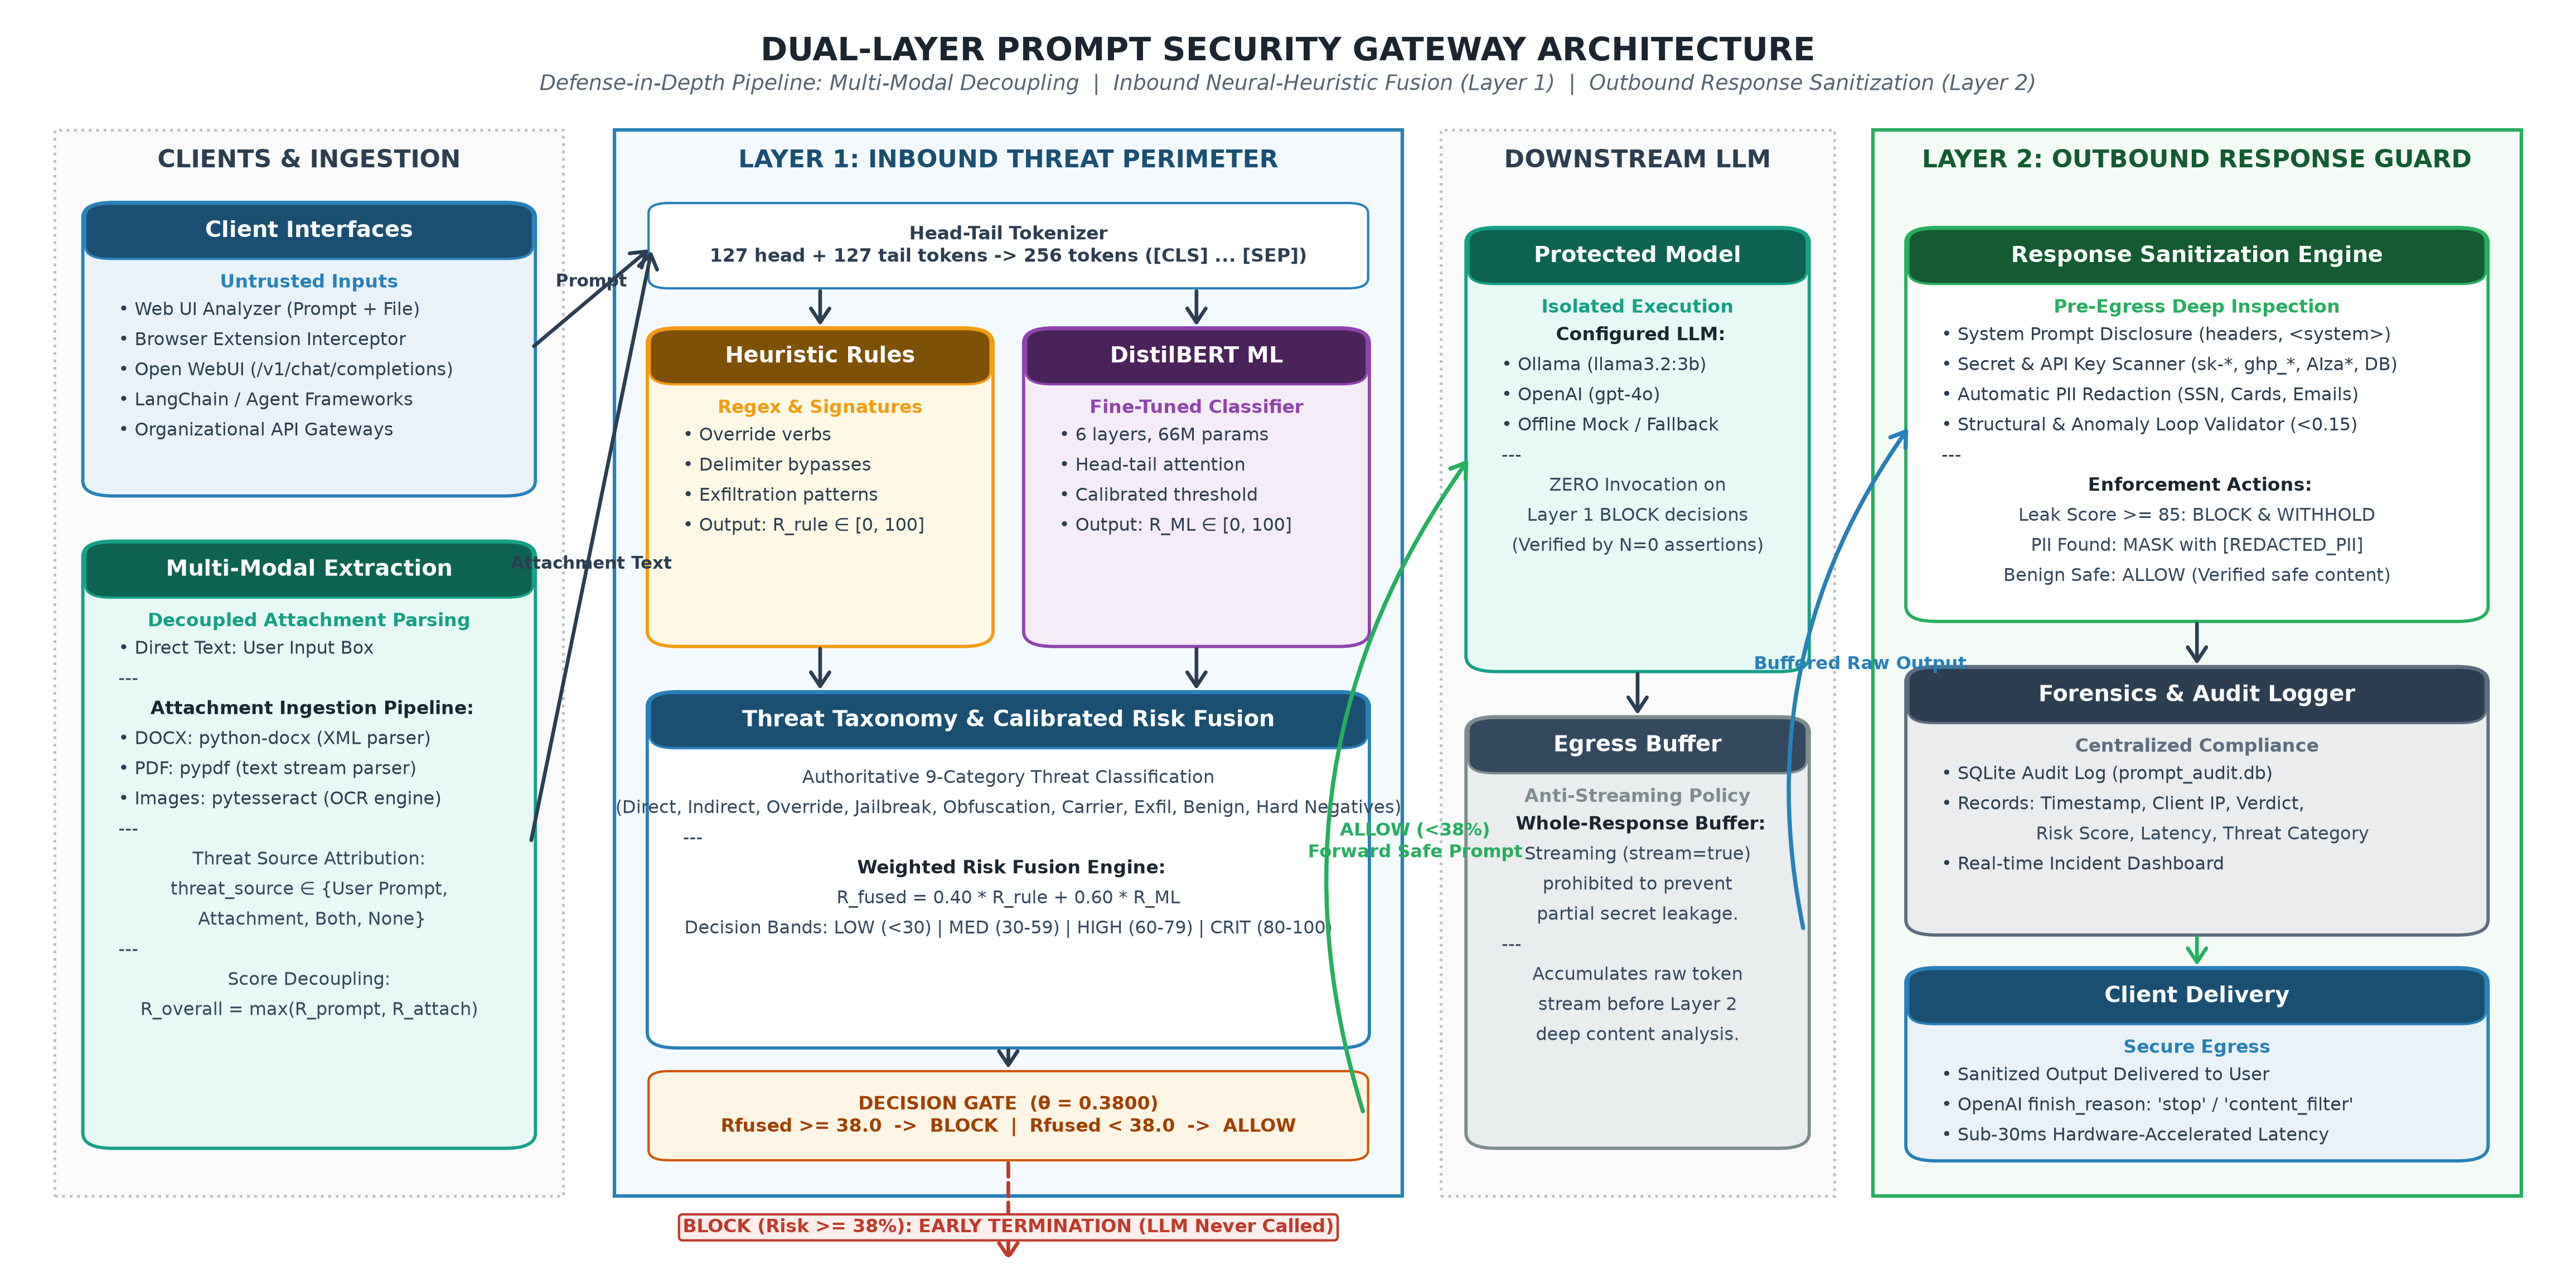
\includegraphics[width=0.95\textwidth]{extracted_im1.png}
\caption{Dual layer prompt-security gateway architecture with multimodal attachment extraction, inbound neural--heuristic blocking, gate pre-execution, response buffering, outbound sanitization, and audit logging.}
\label{fig:architecture}
\end{figure*}

\section{System Architecture and Implementation}
As shown in Fig.~\ref{fig:architecture} the principal request and response path is followed. Input is filtered prior to passing to the downstream LLM, and the output is again checked before it is passed to the client. There's a gateway and a browser extension in the repository, but for the purposes of this paper only behaviors supported by the implementation and tests described below will be evaluated.

\subsection{Input Normalization and Head--Tail Tokenization}
The implementation of the preprocesser will not only keep the starting of a long input but also the ending. As applied, it merges a 127-token head, a 127-token tail, plus the two special tokens for a maximum length of 256 tokens:
\begin{equation}
T_{\text{input}} = [\text{CLS}, t_1, \dots, t_{127}, t_{N-126}, \dots, t_N, \text{SEP}].
\end{equation}
This policy may retain the first and final lines of a text, and may lose the middle of it. This is truncation, not representation of all hidden or distributed instructions.

\subsection{Inbound Layer 1: Neural--Heuristic Screening}
The Inbound Layer 1 is: Neural--Heuristic Screening. Layer 1 fuses rule signals from deterministic rules with an optimised DistilBERT model classifier. Let $R_{\text{rule}}$ be the risk score obtained from the rule and let $P_{\text{mal}}$ be the estimated malicious probability obtained by the classifier. It is indicated by the model score $R_{\text{ML}} = 100 P_{\text{mal}}$. The fused score is calculated as:
\begin{equation}
R_{\text{fused}} = 0.40 R_{\text{rule}} + 0.60 R_{\text{ML}}.
\end{equation}
There are severity based overrides that complement the fusion policy. High severity evidence of attacks can be punishable with a risk floor of 85, and safe cases with hard negative evidence can be capped at a score of 25. The calibrated decision bands will be mapped as: scores $\le 30$ will be mapped to ALLOW, scores between 31 to 60 will be mapped to WARNING and scores $> 60$ will be mapped to BLOCK with the appropriate severity taking precedence. The 0.3800 is a classifier decision threshold and is not used as a final risk-score threshold. Fused scores, severity overrides, and decision bands combine to give defense in depth: the classifier is able to see more broad language patterns, whereas the deterministic rules give interpretable evidence and explicit handling in high severity cases.

When a critical malicious prompt is detected, the backend sends an automated email notification to an integrated Gmail account via SMTP. The alert payload specifies the detected prompt text, its computed risk score, the classified threat category, and the enforcement action taken, notifying administrators in real time.



\subsection{Attachment Parsing and Attribution}
There are two methods of attaching: Parsing and Attribution. The attachment handler can process PDF, DOCX, TXT, legacy DOC and PNG/JPG/JPEG images. The PDF text is extracted using a parser and the DOCX text is extracted from paragraphs and tables. The images are then processed by PDF to Text with OCR and Tesseract and Pillow. LibreOffice is used to convert the old-style DOC files into PDF. The quality of extracted files depends on the structure of files and content quality.

suspicious text in a file is identified with user's request, and text and extracted attachment text are considered as different inputs to prompt. Records descriptive labels for prompt, attachment or combined cases, and applies risk handling with regards to attachments. Also, the simplified expression $R_{\text{overall}} = \max(R_{\text{prompt}}, R_{\text{attachment}})$ doesn't represent all application behavior including attachment specific risk floor and propagation of evidence. The implementation should thus be seen as part of a decision pipeline, rather than a pipe with a single maximum operation. All PDF metadata streams or steganographic content, all embedded XML streams in random or arbitrary XML payloads, are not explicitly claimed herein to be covered by the present parser.

\subsection{Outbound Layer 2: Response Inspection}
Once an allowed request is sent to a configured LLM provider or a test mock, the response is checked before it's sent back to the client. The checked implementation consists of the following classes of checks:
\begin{itemize}
    \item Suspected prompt disclosure: system-prompt or system-markup pattern-based checks. In some cases, High Risk matches may result in the withholding of the response.
    \item Credential-like strings: pattern matching for specified API-key or bearer token, private-key markers, and database connection strings.
    \item PII patterns: masking of certain patterns like credit card numbers, email addresses, SSN numbers and strings with similar patterns per configured rules.
    \item Structural controls: response length bounds, heuristic for repetitive or low diversity output.
\end{itemize}
These are pattern based controls. They may fail to recognize novel formats, and they can also mark benign strings; complete secret detection and zero leakage are not guaranteed in arbitrary deployments by successful synthetic tests.

\subsection{Gateway and Browser Extension}
The Gateway and Browser Extension are not the same. The repository exposes an OpenAI-compatible chat-completions route, for integration with compatible clients. For Layer 2, it is a requirement to inspect the full response before it can be delivered, so an unbuffered token egress is rejected by the gateway. The tests reviewed show that a streaming request can be buffered, checked, and then sent out as a server-sent event (SSE); it would be wrong to take that as a blanket prohibition for all requests with \texttt{stream=true}. The security property is, that no response token must be emitted before the decision on the inspection.

A Chromium browser extension is also provided to capture prompt submission in supported web interfaces and added to the repository. Extension behavior is influenced by page structure, event handling, and cannot be generalized to all websites or browser applications.

\section{Dataset Lineage and Model Provenance}

\begin{table}[t]
\caption{DATASET FILES REPORTED IN THE REPOSITORY}
\label{tab:datasets}
\centering
\begin{tabular}{lrrrl}
\toprule
\textbf{File / split} & \textbf{Rows} & \textbf{Benign} & \textbf{Malicious} & \textbf{Reported role} \\
\midrule
\texttt{train.csv} & 14,317 & 6,979 & 7,338 & Phase 1 training split \\
\texttt{validation.csv} & 3,068 & 1,496 & 1,572 & Phase 1 validation split \\
\texttt{test.csv} & 3,069 & 1,496 & 1,573 & Phase 1 test split \\
\texttt{train\_generalization.csv} & 15,500 & 7,750 & 7,750 & Phase 2 training split \\
\texttt{validation\_generalization.csv} & 3,000 & 1,500 & 1,500 & Phase 2 validation split \\
\texttt{test\_generalization.csv} & 3,000 & 1,500 & 1,500 & Generalization benchmark \\
\texttt{train\_v3.csv} & 16,224 & 8,112 & 8,112 & V3 training corpus \\
\texttt{validation\_v3.csv} & 1,500 & 750 & 750 & V3 validation split \\
\texttt{challenge\_holdout.csv} & 600 & 300 & 300 & Challenge holdout \\
\texttt{hard\_negatives\_expanded.csv} & 300 & 150 & 150 & Expanded hard-negative set \\
\texttt{hard\_negatives\_curated.csv} & 300 & 150 & 150 & Curated hard-negative set \\
\texttt{short\_prompt\_eval.csv} & 200 & 100 & 100 & Short-prompt evaluation \\
\bottomrule
\end{tabular}
\end{table}
The project uses a finalized, balanced V3 training corpus containing 16,224 examples, together with a 1,500-example V3 validation split. The model is evaluated on a separate 3,000-example generalization holdout representing the project's nine-category threat taxonomy. The repository also retains earlier dataset-development stages and targeted evaluation sets for challenge, hard-negative, and short-prompt testing. Table~\ref{tab:datasets} summarizes the documented dataset files and their roles.

The V3 training and validation splits are balanced between benign and malicious examples. The 3,000-example generalization holdout is used to compare the rule-only, DistilBERT-only, and hybrid approaches, while the challenge and hard-negative sets provide targeted checks under distinct input conditions. The model-integrity module records the expected SHA-256 digest \texttt{c15a14cad0bdc9fa909a52c667bff9430e098aebb7c11b375df3d50ae1f0ea93}. The implementation also records the production classifier threshold as 0.3800. These identifiers allow the model artifact and its inference policy to be documented alongside the evaluation results.

\begin{table*}[t]
\caption{DETECTION RESULTS RECOMPUTED FROM REPORTED CONFUSION MATRICES}
\label{tab:results}
\centering
\begin{tabular}{llrrrrrrc}
\toprule
\textbf{Dataset ($N$)} & \textbf{Method} & \textbf{TN} & \textbf{FP} & \textbf{FN} & \textbf{TP} & \textbf{Accuracy} & \textbf{Precision} & \textbf{Recall / F1} \\
\midrule
Generalization (3000) & Rule-only, $> 30$ & 1500 & 0 & 1369 & 131 & 54.37\% & 100.00\% & 8.73\% / 0.1606 \\
Generalization (3000) & Rule-only, $> 60$ & 1500 & 0 & 1375 & 125 & 54.17\% & 100.00\% & 8.33\% / 0.1538 \\
Generalization (3000) & DistilBERT only & 1489 & 11 & 27 & 1473 & 98.73\% & 99.26\% & 98.20\% / 0.9873 \\
Generalization (3000) & Hybrid & 1489 & 11 & 18 & 1482 & 99.03\% & 99.26\% & 98.80\% / 0.9903 \\
\midrule
Challenge (600) & Rule-only, $> 30$ & 300 & 0 & 280 & 20 & 53.33\% & 100.00\% & 6.67\% / 0.1250 \\
Challenge (600) & DistilBERT only & 300 & 0 & 7 & 293 & 98.83\% & 100.00\% & 97.67\% / 0.9882 \\
Challenge (600) & Hybrid & 300 & 0 & 5 & 295 & 99.17\% & 100.00\% & 98.33\% / 0.9916 \\
\midrule
Hard negatives (300) & Rule-only, $> 30$ & 144 & 6 & 141 & 9 & 51.00\% & 60.00\% & 6.00\% / 0.1000 \\
Hard negatives (300) & DistilBERT only & 133 & 17 & 10 & 140 & 91.00\% & 89.17\% & 93.33\% / 0.9121 \\
Hard negatives (300) & Hybrid & 137 & 13 & 7 & 143 & 93.33\% & 91.67\% & 95.33\% / 0.9346 \\
\bottomrule
\end{tabular}
\end{table*}

\section{Experimental Evaluation}
This section compares the rule-only, DistilBERT-only, and hybrid methods using the project evaluation confusion matrices. We define accuracy as $(TP + TN) / N$, precision as $TP / (TP + FP)$, recall as $TP / (TP + FN)$, and F1 as the harmonic mean of precision and recall. The reported datasets are balanced, so accuracy should be read alongside precision, recall, and the confusion counts. We do not claim that the datasets are representative of all real-world prompts.

\subsection{RQ1: Component Comparison}
On the 3,000-example generalization benchmark, the hybrid method reaches 99.03\% accuracy, 99.26\% precision, 98.80\% recall, and F1 of 0.9903. The neural-only baseline reaches 98.73\% accuracy, 99.26\% precision, 98.20\% recall, and F1 of 0.9873. The rule-only baselines have high precision on this benchmark but recall below 9\%, illustrating that the selected rules alone miss many malicious examples in this dataset.

On the challenge holdout, the hybrid method records 5 false negatives and no false positives. As the holdout contains only 300 benign samples, zero observed false positives is a finite-sample observation, not evidence of a universal zero false-positive rate.

On the 300-example hard-negative set used for the table, the hybrid confusion matrix is TN=137, FP=13, FN=7, TP=143. This corresponds to 93.33\% accuracy, 91.67\% precision, 95.33\% recall, and F1 of approximately 0.9346. The hard-negative results shown here correspond to the curated hard-negative evaluation set.

\subsection{RQ2: Attachment Processing}
The project reports placement tests on the challenge set: 50 tail-injection examples with no misses, 25 head-injection examples with 5 misses, and 25 long benign documents with no false positives. These targeted tests exercise attachment-carried instructions at both the beginning and end of long content, alongside benign long-document inputs. Dedicated repository tests also exercise DOCX extraction and image OCR.

\subsection{RQ3: Application Gating and Regression Tests}
The reported automated suite contains 288 passing tests across 20 listed modules, with no reported failures or skips and a reported execution time of 458 seconds. The listed module counts sum to 288. Integration tests use assertions to verify that a blocked request does not invoke the downstream LLM. These integration assertions verify that blocked requests are terminated before downstream model invocation in the tested block paths. The regression suite also validates alert routing in \texttt{test\_detection.py}, verifying that safe queries skip notification whereas critical malicious prompts trigger automated Gmail alert dispatch, as demonstrated during Review 3.

\subsection{RQ4: Outbound Response Checks}
The project reports synthetic tests in which credential-like strings were intercepted and withheld, selected PII patterns were masked, and benign sample responses were allowed. These tests demonstrate the configured response-handling behavior for the evaluated synthetic cases, including withholding credential-like outputs and masking selected PII patterns before delivery.

\subsection{Latency}
The reported Layer 1 timing totals are 29.3 ms on Apple MPS, 22.7 ms on CUDA, and 84.7 ms on x86 CPU. Adding the two listed Layer 2 inspection stages gives approximate security-middleware totals of 33.4 ms, 26.5 ms, and 89.3 ms, respectively. These sums exclude downstream LLM generation, network transfer, attachment parsing/OCR, and any queueing or deployment overhead. They should therefore be described as measured pipeline-stage latency, not end-to-end user response latency.

\section{Discussion}
The benchmark results demonstrate that the neural and hybrid methods perform significantly better than the rule-only baseline methods on the tested sets in terms of the number of malicious examples correctly identified. It also reveals that the hybrid detector has no ability to block false positives: in the confusion matrix presented, 13 out of 150 instances of benign examples were reported as harmful. Such a trade-off is important for actual deployments where blocking a legitimate request can come with a price. This comparison can be expanded to other deployment conditions by extending the range of evaluation with respect to attack type, language, prompt length and application context.

It's a two-layer design that covers two points of failure. Inbound screening can filter out suspicious requests from before the model is invoked, thus decreasing the number of calls for blocked inputs. Selected leakage patterns in responses may be picked up on at a second opportunity through outbound inspection. In neither case is the layer complete: in either, the classifier can be outmoded, the patterns can be incomplete, the attachments can be missing, and the response filters can be missing the new or semantically expressed disclosures. Therefore, defense in depth is more about risk reduction rather than an assurance that attacks cannot be successful.

\subsection{Streaming and Egress Policy}
Response inspection must occur before sensitive content is sent to the client if the system is expected to withhold or redact the complete response. The reviewed gateway tests support buffering a response, inspecting it, and then emitting it as SSE where requested. The security requirement is thus to prevent uninspected token egress, not necessarily to ban the API's streaming option altogether. This introduces a latency and memory trade-off that should be measured under realistic response sizes and concurrent loads.

\section{Limitations and Responsible Use}
The detector's measured performance is tied to the evaluated datasets and does not imply that every prompt-injection attempt will be detected. The rule engine can miss paraphrased attacks, the classifier may encounter distribution shift, and head tail tokenization can omit relevant material from the middle of long inputs. Attachment extraction and OCR quality depend on file structure, image resolution, and contrast. Outbound filters use configured patterns and heuristics, so they may miss unfamiliar secret formats or flag benign lookalikes. The browser extension's behavior depends on the structure of supported web interfaces. These components are intended as defense-in-depth controls and should be combined with least-privilege tool access, secure secret management, monitoring, and appropriate incident handling.

\section{Conclusion}
This paper proposed a dual-layer security design for prompt-injection defense, which includes neural--heuristic fusion, multimodal attachment parsing, pre-execution gating and outbound leakage prevention. The hybrid detector has 99.03\% accuracy, 99.26\% precision, 98.80\% recall and an F1 score of 0.9903 on the 3,000 example generalization holdout. It achieves 99.17\% accuracy and 98.33\% recall on the 600-example challenge holdout, with no false positives in the 300 benign examples. It has an accuracy of 93.33\% and a recall of 95.33\% on the curated hard-negative set of 300 examples, and it flags 13 benign examples. There are 288 regression tests in 20 modules for the implementation. Reported latency is 22.7 ms on CUDA, 29.3 ms on Apple MPS, and 84.7 ms on CPU (excluding downstream LLM generation); the listed latency for Layer 1 and Layer 2 stages add up to 26.5 ms, 33.4 ms, and 89.3 ms, respectively.

The results show the usefulness of the neural classifier and interpretable rules and a separate response-inspection layer. For block paths that are tested, requests are blocked before the downstream model is invoked and completed responses are checked before delivery. The architecture thus offers complementary controls at the input and output boundaries of LLM applications.





\begin{table}[t]
\caption{AUTOMATED TEST SUITE SUMMARY}
\label{tab:tests}
\centering
\begin{tabular}{lcp{4.2cm}}
\toprule
\textbf{Subsystem / test module} & \textbf{Tests} & \textbf{Coverage described by the repository} \\
\midrule
Admin authentication & 30 & Password hashing, sessions, admin security \\
Attachments & 34 & PDF/DOCX extraction, size limits, attachment gating \\
Image OCR attachments & 19 & Tesseract OCR and image-carried content \\
Block-dialog UI & 13 & Modal behavior and responsive actions \\
Detection & 14 & Layer 1 decisions, threshold behavior, edge cases \\
DOCX indirect injection & 4 & DOCX carrier injection and pre-invocation gating \\
Dual-layer integration & 6 & Layer 1/Layer 2 decision propagation \\
Extension interception & 15 & Browser DOM interception and concurrency locks \\
Extension parity & 28 & Extension/API verdict consistency \\
External LLM demo & 9 & Provider client, failover, model selection \\
Integration center & 9 & Metadata, connection tests, incident filtering \\
Layer 2 demo & 16 & Response inspection and synthetic leak handling \\
LLM client & 6 & Provider routing and local mock \\
Model integrity & 25 & Checkpoint digest validation and fallback behavior \\
Open WebUI deployment & 8 & Reverse-proxy integration checks \\
OpenAI gateway integration & 12 & Chat-completions schema and streaming behavior \\
Scenarios A--H & 10 & End-to-end scenario checks \\
Nine-category taxonomy & 14 & Taxonomy classification and fallback \\
UI navigation and themes & 7 & Navigation and theme behavior \\
Web UI integration & 9 & Routes, dashboard, incident logging \\
\midrule
\textbf{Total} & \textbf{288} & \textbf{20 listed modules; 288 reported passing tests} \\
\bottomrule
\end{tabular}
\end{table}

\begin{table}[t]
\caption{REPORTED SECURITY-MIDDLEWARE LATENCY BY RUNTIME}
\label{tab:latency}
\centering
\begin{tabular}{lrrr}
\toprule
\textbf{Pipeline stage} & \textbf{MPS} & \textbf{CUDA} & \textbf{CPU} \\
\midrule
Preprocessing & 1.1 & 1.0 & 1.8 \\
Rule engine & 3.2 & 3.1 & 3.9 \\
DistilBERT inference & 24.6 & 18.2 & 78.4 \\
Decision gate & 0.4 & 0.4 & 0.6 \\
\textbf{Layer 1 subtotal} & \textbf{29.3} & \textbf{22.7} & \textbf{84.7} \\
Layer 2 regex / PII & 3.8 & 3.5 & 4.2 \\
Layer 2 validation & 0.3 & 0.3 & 0.4 \\
\textbf{Combined listed stages} & \textbf{33.4} & \textbf{26.5} & \textbf{89.3} \\
\bottomrule
\multicolumn{4}{p{0.45\textwidth}}{\footnotesize Values are in milliseconds. Combined values sum the listed Layer 1 and Layer 2 stages and exclude LLM generation and other unmeasured overhead.}
\end{tabular}
\end{table}

\section*{Acknowledgment}
The authors acknowledge the guidance of Mrs. Usha Anirudhha Jogalekar, Assistant Professor, Department of Computer Science \& Engineering, Symbiosis Institute of Technology, Symbiosis International (Deemed University), Pune, India.

\begin{thebibliography}{00}
\bibitem{b1} F. Perez and I. Ribeiro, ``Ignore previous prompt: Attack techniques for language models,'' \emph{arXiv:2211.09527}, 2022.
\bibitem{b2} K. Greshake, S. Abdelnabi, S. Mishra, C. Endres, T. Holz, and M. Fritz, ``Not what you've signed up for: Compromising real-world LLM-integrated applications with indirect prompt injection,'' in \emph{Proc. ACM Workshop on Artificial Intelligence and Security}, 2023, pp. 79--90, doi: 10.1145/3605764.3623985.
\bibitem{b3} Y. Liu, G. Deng, Y. Li, K. Wang, Z. Wang, X. Wang, T. Zhang, Y. Liu, H. Wang, Y. Zheng, L. Y. Zhang, and Y. Liu, ``Prompt injection attack against LLM-integrated applications,'' \emph{arXiv:2306.05499}, 2023.
\bibitem{b4} Q. Zhan, Z. Liang, Z. Ying, and D. Kang, ``InjecAgent: Benchmarking indirect prompt injections in tool-integrated large language model agents,'' in \emph{Findings of the Association for Computational Linguistics: ACL 2024}, 2024, pp. 10471--10506, doi: 10.18653/v1/2024.findings-acl.624.
\bibitem{b5} E. Debenedetti, J. Zhang, M. Balunovic, L. Beurer-Kellner, M. Fischer, and F. Tram`er, ``AgentDojo: A dynamic environment to evaluate prompt injection attacks and defenses for LLM agents,'' in \emph{Advances in Neural Information Processing Systems}, vol. 37, 2024.
\bibitem{b6} G. Kholkar and R. Ahuja, ``CAPTURE: Context-aware prompt injection testing and robustness enhancement,'' in \emph{Proc. 1st Workshop on LLM Security}, 2025, pp. 176--188.
\bibitem{b7} C. Cui, Y. Wu, M. Backes, and Y. Zhang, ``Rethinking assessments of prompt injection attacks,'' in \emph{Findings of the Association for Computational Linguistics: ACL 2026}, 2026, pp. 23773--23799, doi: 10.18653/v1/2026.findings-acl.1191.
\bibitem{b8} K. Zhu, J. Wang, J. Zhou, Z. Wang, H. Chen, Y. Wang, L. Yang, W. Ye, Y. Zhang, N. Z. Gong, and X. Xie, ``PromptRobust: Towards evaluating the robustness of large language models on adversarial prompts,'' \emph{arXiv:2306.04528}, 2023.
\bibitem{b9} V. Sanh, L. Debut, J. Chaumond, and T. Wolf, ``DistilBERT, a distilled version of BERT: Smaller, faster, cheaper and lighter,'' \emph{arXiv:1910.01108}, 2019.
\bibitem{b10} N. Carlini et al., ``Extracting training data from large language models,'' in \emph{Proc. 30th USENIX Security Symposium}, 2021, pp. 2633--2650.
\bibitem{b11} C. Autio et al., ``Artificial intelligence risk management framework: Generative artificial intelligence profile,'' NIST AI 600-1, 2024, doi: 10.6028/NIST.AI.600-1.
\bibitem{b12} OW ASP GenAI Security Project, ``OW ASP Top 10 for Large Language Model Applications and Generative AI 2025,'' OW ASP Foundation, 2025. [Online]. Available: \url{https://owasp.org/www-project-top-10-for-large-language-model-applications/}
\end{thebibliography}

\end{document}
